\documentclass[compress]{beamer}
\usepackage[T1]{fontenc}
\usepackage[utf8]{inputenc}
\usepackage[italian]{babel}
\usepackage{array} % needed for \arraybackslash
\usepackage{graphicx}
\usepackage{adjustbox} % for \adjincludegraphics
\usepackage{soul}
\usepackage{color}
\usepackage{animate}

\usepackage{../Manoscritto/Styles/commands}

\newcommand{\nota}[1]{\textcolor{red}{#1}}

\title[]{Tensor Train Decomposition:\\ a tensor representation format for high-dimensional problems}
\author{Tommaso Bianucci}
\date{9 Giugno 2017}
\institute{Università di Pisa}
%\logo{\includegraphics[width=15mm]{logo}}
\usetheme{Dresden}
%\usecolortheme{wolverine}
%\useoutertheme[right]{sidebar}
\setbeamercovered{dynamic}
\setbeamertemplate{theorems}[numbered]
\theoremstyle{definition}
\newtheorem{definizione}{Definizione}
\theoremstyle{plain}
\newtheorem{teorema}{Teorema}

\begin{document}

\begin{frame}
\maketitle
\end{frame}

\section{Tensori}
\subsection{Introduzione}
\begin{frame}
\frametitle{Cosa sono i Tensori?}
\begin{itemize}
\item Array multidimensionali
\item Generalizzazione di vettori e matrici
\end{itemize}
\vspace{1mm}
\begin{center}
	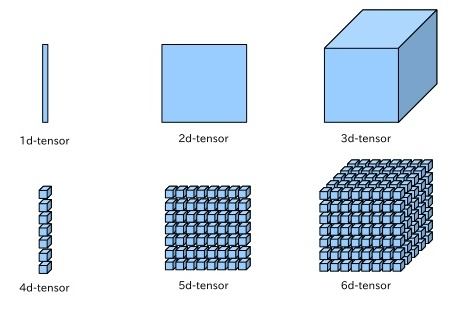
\includegraphics[width=0.6\textwidth]{Img/tensors.jpg}
\end{center}
\end{frame}

\begin{frame}
\frametitle{Interesse e applicazioni}
I tensori trovano applicazione in contesti ad elevata dimensionalità, come:
\begin{itemize}
\item Deep Learning
\item Analisi di segnali
\item Fisica e chimica computazionali
\item Soluzione di PDE
\end{itemize}
\end{frame}

\begin{frame}
\frametitle{Curse of dimensionality}
I tensori sono ingombranti: \alert{$n \times n \times \cdots \times n \rightarrow n^d$}
\begin{itemize}
\item Aumento esponenziale del numero di elementi rispetto alla dimensionalità
\item Raggiungiamo facilmente i limiti fisici del calcolatore
\end{itemize}

% \vspace{5mm}
% $\longrightarrow$ \emph{Curse of dimensionality}
\end{frame}	

\subsection{Definizioni e strumenti}
\begin{frame}
\frametitle{Definizioni e strumenti}
\begin{itemize}
\item Fibre e fette
\item Unfolding
\item Rango
\item SVD
\end{itemize}
\end{frame}

\begin{frame}
\frametitle{Fibre e fette}
Le \emph{fibre} di un tensore sono vettori di elementi ottenute fissando tutti gli indici tranne uno.
Analoghe a righe e colonne nelle matrici.

\begin{center}
	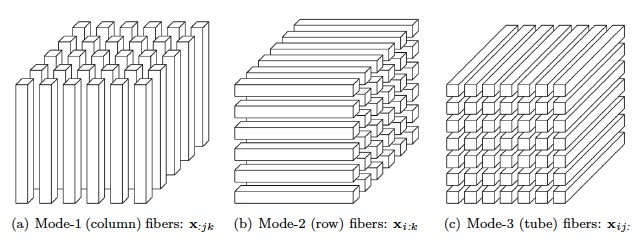
\includegraphics[width=0.4\textwidth]{Img/fibers.jpg}
\end{center}

\pause
Le \emph{fette} di un tensore sono matrici di elementi ottenute fissando tutti gli indici tranne due.

\begin{center}
	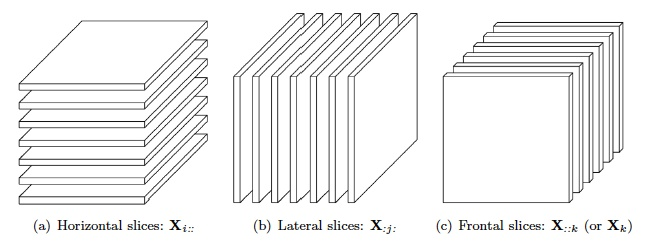
\includegraphics[width=0.4\textwidth]{Img/slices.jpg}
\end{center}
\end{frame}

\begin{frame}
\frametitle{Unfolding}
\emph{Unfolding} o \emph{matricizzazione} è il processo di riportare gli elementi di un tensore su una matrice.

\begin{center}
	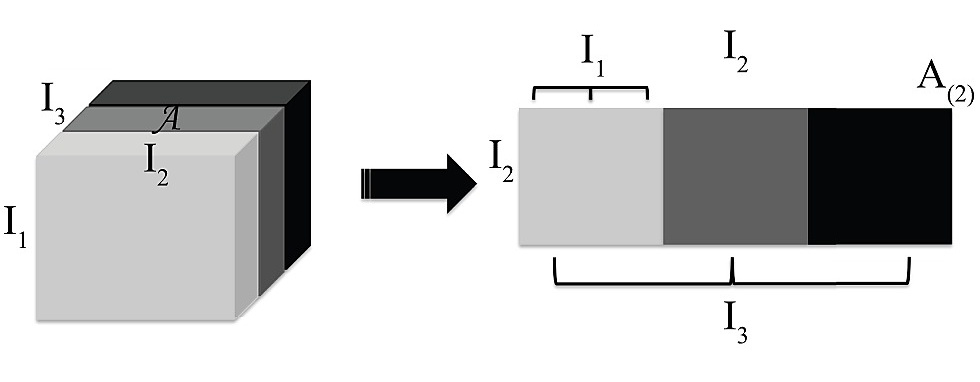
\includegraphics[width=0.5\textwidth]{Img/unfolding.jpg}
\end{center}

\pause
Preso un tensore \A, il \emph{$k$-esimo unfolding} è dato dal considerare i primi k indici e i restanti come due multi-indici:
\begin{equation*}
	A_k = A_k(
	\underbrace{I}_{i_1,\dots,i_k}
	,
	\underbrace{J}_{i_{k+1},\dots,i_d}
	) = A(i_1,\dots,i_d)	
\end{equation*}
\end{frame}

\begin{frame}
\frametitle{Rango}
Il \emph{rango} di un tensore è il minimo numero di tensori \emph{rango-$1$} la cui somma dà il tensore di partenza.

\pause
\vspace{5mm}
Un $d$-tensore di \emph{rango} $1$ è il risultato del prodotto esterno di $d$ vettori:

\begin{columns}
\begin{column}{0.5\textwidth}
\begin{equation*}
  \A = v^{(1)} \circ v^{(2)} \circ \cdots \circ v^{(d)}
\end{equation*}

\begin{equation*}
  a_{i_1,i_2,\ldots,i_d} = v_{i_1}^{(1)} v_{i_2}^{(2)} \cdots v_{i_d}^{(d)}
\end{equation*}
\end{column}

\begin{column}{0.5\textwidth}
\begin{center}
	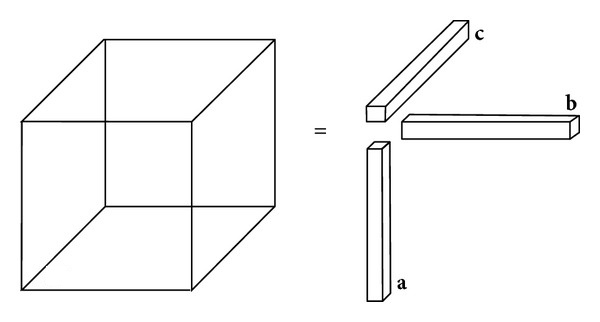
\includegraphics[width=0.8\textwidth]{Img/rank_one_tensor.jpg}
\end{center}
\end{column}
\end{columns}
\end{frame}

\begin{frame}
\frametitle{Decomposizione a valori singolari (SVD)}
La SVD ci permette di fattorizzare una matrice $A$ in:
\begin{equation*}
	A = U \Sigma V^T
\end{equation*}
\begin{itemize}
	\item $U$ e $V$ sono matrici ortonormali
	\item $\Sigma$ è matrice diagonale	
	\item Elementi di $\Sigma$ sono $\sigma_1 > \sigma_2 > \cdots > \sigma_r > 0$
	\item \emph{Troncando} $\Sigma$ otteniamo approssimazione di rango minore
\end{itemize}
\end{frame}

\subsection{Decomposizioni}
\begin{frame}
\frametitle{Decomposizioni di tensori}
Storicamente le decomposizioni principali presentate sono state: 

\vspace{5mm}
\begin{columns}
\begin{column}{0.6\textwidth}
\begin{itemize}
\item CANDECOMP/PARAFAC (CP) %\\
	% $\A \approx \sum_{r = 1}^R a_r^{(1)} \circ a_r^{(2)} \circ \cdots \circ a_r^{(d)}$
	\vspace{3mm}
\item Tucker
\end{itemize}
\end{column}
\begin{column}{0.4\textwidth}
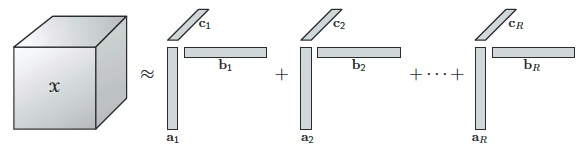
\includegraphics[width=0.85\textwidth]{Img/cp.jpg}

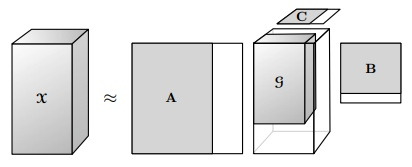
\includegraphics[width=0.7\textwidth]{Img/tucker.jpg}
\end{column}
\end{columns}

\vspace{5mm}
Teoricamente valide, ma computazionalmente problematiche:
\begin{itemize}
	\item Mancanza di algoritmi di decomposizione stabili.
	\item Dipendenza esponenziale del numero di parametri rispetto alla dimensionalità del tensore.
\end{itemize}
\end{frame}

\section{Tensor Train}
\subsection{Tensor Train}
\begin{frame}
\frametitle{Una decomposizione migliore è possibile?}
Vorremmo una decomposizione computazionalmente maneggevole:
\begin{itemize}
\item La memoria occupata non deve dipendere esponenzialmente dalla dimensionalità del tensore (fissato l'errore)
\item Deve avere un algoritmo di approssimazione e decomposizione stabile
\item Necessario poter eseguire le operazioni di algebra lineare di base direttamente nel formato \emph{compresso}
\end{itemize}
\end{frame}

\begin{frame}
\frametitle{Tensor Train Decomposition (TT)}
$\A$ tensore $d$-dimensionale, $\G_i$ \emph{core} $3$-dimensionali:
\begin{equation*}
	\A = 
	\underbrace{\G_1}_{1 \times n_1 \times r_1} 
	\times 
	\underbrace{\G_2}_{r_1 \times n_2 \times r_2} 
	\times 
	\cdots 
	\times 
	\underbrace{\G_d}_{r_{d-1} \times n_d \times 1}
\end{equation*}
Otteniamo ogni elemento del tensore tramite moltiplicazione delle matrici $G_k(i_k)$\,:
\begin{equation*}
	\A(i_1,i_2,\dots,i_d) = 
	\underbrace{G_1(i_1)}_{1 \times r_1}
	\underbrace{G_2(i_2)}_{r_1 \times r_2}
	\cdots
	\underbrace{G_d(i_d)}_{r_{d-1} \times 1}
\end{equation*}

% \begin{center}
% 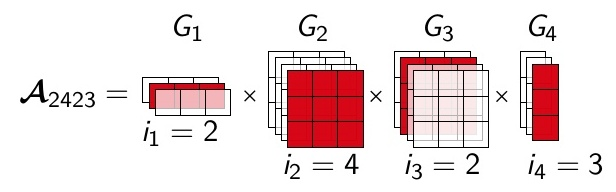
\includegraphics[width=0.5\textwidth]{Img/tt_example.jpg}
% \end{center}
Ad esempio: $\A(2,4,2,3) = \raisebox{-0.5\height}{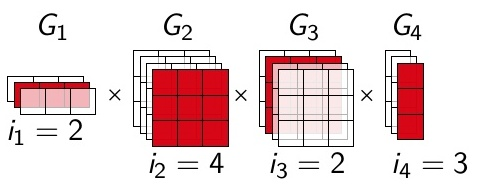
\includegraphics[width=0.4\textwidth]{Img/tt_example_2.jpg}}$
\end{frame}

\subsection{Calcolo}
\begin{frame}
\frametitle{Come calcolare la TT?}
%Abbiamo alcuni risultati:
\begin{teorema}[Oseledets, 2011]
Sia \A un $d$-tensore e sia, per ogni $k$, $A_k$ il $k$-esimo unfolding.
Allora esiste una decomposizione TT con ranghi $r_k^{(tt)}$ t.c. $r_k^{(tt)} \leq rk(A_k) \, \forall k$
\end{teorema}

\vspace{5mm}
La dimostrazione di questo teorema:
\begin{itemize}
	\item \`E costruttiva
	\item Fornisce l'algoritmo \emph{TT-SVD}
	\item \`E basata sull'approssimazione delle matrici di unfolding
\end{itemize}
\end{frame}

\begin{frame}
\frametitle{Come calcolare la TT? (2)}
\begin{teorema}[Oseledets, 2011]
Poniamo che gli unfolding $A_k$ di \A abbiano $\epsilon$-rango $r_k$.
Allora l'algoritmo TT-SVD produce un tensore \B in formato TT, con ranghi $r_k$ e t.c. 
\begin{equation*}
    ||\A - \B ||_F \le \epsilon \sqrt{d-1}\, .
\end{equation*}
\end{teorema}

\vspace{5mm}
Questo risultato:
\begin{itemize}
	\item Assicura la stabilità dell'algoritmo TT-SVD
	\item Fornisce la soglia di approssimazione sulle SVD per ottenere la precisione desiderata sulla TT
\end{itemize}
\end{frame}

\begin{frame}
\frametitle{TT-SVD in pillole}
%\nota{Inserisci qui uno schema di base dell'algo TT-SVD}
\begin{enumerate}
	\item Calcoliamo la soglia di troncamento SVD: $\delta = \frac{\epsilon}{\sqrt{d-1}} ||\A||_F$
	\item Per ogni dimensione $k$
		\begin{enumerate}
			\item Facciamo primo unfolding del tensore $\rightarrow C$
			\item Calcoliamo $SVD_{\delta}(C) \rightarrow U,S,V$
			\item Il core corrente $G_k$ è dato dall'opportuno reshape di $U$
			\item Procediamo considerando come tensore il reshape di $SV^T$
		\end{enumerate}
\end{enumerate}
\end{frame}

\subsection{Operazioni in TT}
\begin{frame}
\frametitle{Rounding e algebra lineare}
\`E possibile \emph{arrotondare} ad una nuova precisione un tensore in formato TT:
\begin{itemize}
	\item \emph{Rounding}
\end{itemize}

\pause
\vspace{3mm}
Le operazioni di algebra lineare sono facilmente calcolabili in formato TT:
\begin{itemize}
\item Somma
\item Moltiplicazione per scalare
\item Prodotto scalare
\item Norma
\end{itemize}
\end{frame}

\subsection{Numero di parametri}
\begin{frame}
\frametitle{Quanto spazio?}
\begin{equation*}
	TT_\epsilon(\A) = 
	\underbrace{\G_1}_{1 \times n_1 \times r_1}
	\times \cdots \times
	\underbrace{\G_k}_{r_{k-1} \times n_k \times r_k}
	\times \cdots \times 
	\underbrace{\G_d}_{r_{d-1} \times n_d \times 1}
\end{equation*}	

\vspace{5mm}
Se $\,r_k \leq r\,$ e $\,n_k \leq n\,$ per ogni $\,k$, otteniamo:
\begin{equation*}
	2nr + (d-2)nr^2 = \mathcal{O}(dnr^2)
\end{equation*}

Quindi:
\begin{itemize}
	\item Non c'è dipendenza esponenziale dall'ordine del tensore
	\item Dipendenza è principalmente sulla precisione scelta
\end{itemize}
\end{frame}

\subsection{In sintesi}
\begin{frame}
\frametitle{Abbiamo raggiunto i nostri obiettivi?}
\begin{itemize}
\item La memoria occupata non dipende esponenzialmente dal grado del tensore $\rightarrow$ {$\color{blue} \mathcal{O}(dnr^2)$} \color{black}
\item Esiste algoritmo di approssimazione e decomposizione stabile $\rightarrow$ \textcolor{blue}{Teorema 1 + Teorema 2}
\item \`E possibile eseguire le operazioni di algebra lineare di base direttamente nel formato \emph{compresso}
\end{itemize}
\end{frame}

\section{TT-Cross}
\subsection{Oltre i limiti di dimensionalità}
\begin{frame}
\frametitle{Non proprio...}
\pause
\alert{Tutto~funziona~solo~se~possiamo~immagazzinare~il~tensore~di~partenza.}
\end{frame}

\begin{frame}
\frametitle{Approssimazione iterativa di tensori \emph{black-box}}
In alcuni casi possiamo avere un tensore di cui si possano calcolare gli elementi a partire dalle coordinate $\rightarrow$ \emph{black-box}

\vspace{10mm}
Vorremmo poter costruire l'approssimazione TT iterativamente, calcolando e utilizzando solo alcuni elementi alla volta.
\end{frame}

\begin{frame}
\frametitle{TT-Cross}
Possiamo ottenere un tale algoritmo iterativo, chiamato \emph{TT-Cross}, adattando TT-SVD:
\begin{itemize}
	\item Approssimiamo gli unfolding tramite un loro sottoinsieme di righe e di colonne $\rightarrow$ algoritmo \emph{maxvol}
	\item Si dimostra che il numero di elementi da calcolare per approssimare l'intero tensore è $\mathcal{O}(dnr^2)$
\end{itemize}

\vspace{5mm}
(Oseledets, Tyrtyshnikov, 2011)
\end{frame}

\section{Conclusioni}
\subsection{Esempio su immagini}
\begin{frame}
\frametitle{Esempio su immagini}
%\alert{Inseriamo le gif di esempio?}
\begin{columns}
\begin{column}{0.5\textwidth}
	% \animategraphics[loop,width=\linewidth]{10}{Img/cats_orig.d/cats_orig-}{0}{117}
	% \vspace{3mm}
	% \animategraphics[loop,width=\linewidth]{10}{Img/cats_4.d/cats_4-}{0}{117}
	\animategraphics[loop,width=\linewidth]{10}{Img/cats_orig.d/cats_orig-}{45}{70}
	\vspace{3mm}
	\animategraphics[loop,width=\linewidth]{10}{Img/cats_4.d/cats_4-}{45}{70}
\end{column}
\begin{column}{0.5\textwidth}
	% \animategraphics[loop,width=\linewidth]{10}{Img/cats_1.d/cats_1-}{0}{117}
	% \vspace{3mm}
	% \animategraphics[loop,width=\linewidth]{10}{Img/cats_7.d/cats_7-}{0}{117}
		\animategraphics[loop,width=\linewidth]{10}{Img/cats_1.d/cats_1-}{45}{70}
	\vspace{3mm}
	\animategraphics[loop,width=\linewidth]{10}{Img/cats_7.d/cats_7-}{45}{70}
\end{column}
\end{columns}
\end{frame}

\subsection{Conclusioni}
\begin{frame}
\frametitle{Conclusioni}
\begin{itemize}
	\item I tensori sono oggetti che ci permettono di trattare problemi multidimensionali.
	\item La Tensor Train Decomposition ci permette di rendere computazionalmente accessibili questi problemi anche a dimensionalità prima inaccessibili.
	\item L'approccio TT-Cross permette di trattare tensori la cui dimensionalità rende impossibile anche solo immagazzinarne la rappresentazione esplicita.
\end{itemize}

\pause
\vspace{2mm}
\begin{center}
	\Huge Grazie!
\end{center}
\end{frame}

% \subsection{Fine}
% \begin{frame}
% Grazie!
% \end{frame}

\end{document}
